\documentclass[classe=$2^{de}$]{coursclass}

\title{Chapitre 2 : Ensembles de nombres}
\date{}
\author{}

\begin{document}

\maketitle

\section{Ensembles usuels}

\begin{definition}[Entiers]
	\begin{itemize}
		\item Un \uline{nombre entier naturel} est un nombre entier positif ou nul. On note l'ensemble des nombres entiers naturels $ℕ$.
		\item Un \uline{nombre entier relatif} est un nombre entier positif, négatif ou nul. On note l'ensemble des nombres entiers relatifs $ℤ$. % ℤ pour l'allemand "Zahlen"
	\end{itemize}
\end{definition}

\begin{remarque}
	Tout nombre entier naturel est un nombre entier relatif : on note $ℕ ⊂ ℤ$.
\end{remarque}

\begin{definition}[Nombres décimaux et rationnels]
	\begin{itemize}
		\item Un \uline{nombre décimal} est un nombre pouvant s'écrire $\dfrac{a}{10ⁿ}$, où $a$ est un nombre entier relatif et $n$ est un entier naturel. On note l'ensemble des nombres décimaux $𝔻$.
		\item Un \uline{nombre rationnel} est un nombre pouvant s'écrire $\dfrac{a}{b}$, où $a$ est un nombre entier relatif et $b$ est un entier naturel non nul. On note l'ensemble des nombres rationnels $ℚ$. % ℚ pour "quotient"
	\end{itemize}
\end{definition}

\begin{remarque}
	\begin{itemize}
		\item Tout entier relatif est un nombre décimal.
		\item Tout nombre décimal est un nombre rationnel.
	\end{itemize}
	On note $ℕ ⊂ ℤ ⊂ 𝔻 ⊂ ℚ$.
\end{remarque}

\begin{definition}[Nombre réel]
	On a deux manières de définir les nombres réels :
	\begin{itemize}
		\item Si on considére une droite graduée, l'ensemble des abscisses des points de cette droite forme \uline{l'ensemble des nombres réels}.
		\item Alternativement, un \uline{nombre réel} est un nombre qui peut s'écrire comme un entier suivi d'un nombre fini ou infini de chiffres après la virgule.
	\end{itemize}

	\begin{center}
		\begin{tikzpicture}
			\draw[\myArrow] (-5,0) -- (5,0);
			\draw (0,0) -- ++(0,-0.2) node[below] {$0$};
			\draw (1,0) -- ++(0,-0.2) node[below] {$1$};
			\draw (-3,0) -- ++(0,-0.2) node[below] {$-3$};
			\draw (2.41,0) -- ++(0,-0.2) node[below] {$\sqrt{2}$};
			\draw (3.14,0) -- ++(0,-0.2) node[below] {$π$};
		\end{tikzpicture}
	\end{center}

	On note l'ensemble des nombres réels $ℝ$.
\end{definition}

\begin{remarque}
	Tout nombre rationnel est un nombre réel.

	On note $ℕ ⊂ ℤ ⊂ 𝔻 ⊂ ℚ ⊂ ℝ$.
\end{remarque}

\begin{center}
	\begin{tikzpicture}[every node/.style={scale=0.85}]
		\draw (0,0) ellipse (2 and 1);
		\draw (0,0.5) ellipse (3.7 and 2);
		\draw (0,1) ellipse (5.4 and 3);
		\draw (0,1.5) ellipse (7.1 and 4);
		\draw (0,2) ellipse (8.8 and 5);

		\node at (0,0.7) {$ℕ$};
		\node at (-0.9,0.1) {$0$};
		\node at (0,0.1) {$1$};
		\node at (0.9,0.1) {$2$};
		\node at (-0.6,-0.5) {$50$};
		\node at (0.6,-0.5) {$357$ $892$};

		\node at (0,2.2) {$ℤ$};
		\node at (-1,1.7) {$-1$};
		\node at (1.2,1.7) {$-76$};
		\node at (-2.5,0.5) {$-2689$};

		\node at (0,3.7) {$𝔻$};
		\node at (-3,2.7) {$0{,}8$};
		\node at (2,2.8) {$-89{,}127$};

		\node at (0,5.2) {$ℚ$};
		\node at (-6,2) {$-\frac{6}{11}$};
		\node at (-3,4) {$\frac{1}{3}$};
		\node at (5,3.5) {$\frac{60}{859}$};

		\node at (0,6.7) {$ℝ$};
		\node at (-5,5) {$\sqrt{3}$};
		\node at (-2,6) {$\sqrt{2}$};
		\node at (3,6) {$π$};
		\node at (8,3) {$e$};
	\end{tikzpicture}
\end{center}

\begin{exemple}
	\begin{itemize}
		\item Exemple d'entiers naturels : $0$ ; $1$ ; $2$ ; $50$ ; $357$ ; $892$ ...
		\item Exemple d'entiers relatifs mais pas naturels : $-1$ ; $-76$ ; $-2689$ ...
		\item Exemple de nombres décimaux mais pas d'entiers relatifs : $0,8$ ; $-89,127$ ...
		\item Exemple de nombres rationnels mais pas décimaux : $\dfrac{6}{11}$ ; $\dfrac{1}{3}$ ; $\dfrac{60}{859}$ ...
		\item Exemple de nombres réels mais pas rationnels : $\sqrt{2}$ ; $\sqrt{3}$ ; $π$ ; $e$ ...
	\end{itemize}
\end{exemple}

\section{Intervalles}

\begin{definition}[Intervalle de $ℝ$]
	Soient $a$ et $b$ deux nombres réels tels que $a ≤ b$.
	\begin{itemize}
		\item L'\textbf{intervalle} $[a ; b]$ est l'ensemble des nombres réels $x$ tels que $x ≥ a$ et $x ≤ b$.

		      On dit que $a$ et $b$ sont les \textbf{bornes} de cet intervalle.

		      L'\textbf{amplitude} de cet intervalle est $b - a$.
		\item L'\textbf{intervalle} $]-∞ ; b]$ est l'ensemble des nombres réels $x$ tels que $x ≤ b$.
		\item L'\textbf{intervalle} $[a ; +∞[$ est l'ensemble des nombres réels $x$ tels que $x ≥ a$.
	\end{itemize}

	Pour exclure une des bornes d'un intervalle, il faut utiliser un crochet tourné vers l'extérieur.

	Ainsi $[a ; b[$ est l'ensemble des nombres réels $x$ tels que $x ≥ a$ et $x < b$.
\end{definition}

\begin{exemple}
	\begin{center}
		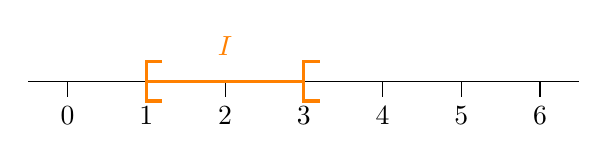
\begin{tikzpicture}
			\draw[\myArrow] (-0.5,0) -- (6.5,0);
			\foreach \x in {0,...,6} {
					\draw (\x,0) -- ++(0,-0.2) node[below] {$\x$};
				}
			\draw[very thick,orange]
			(1,0) -- (3,0)
			(1.2,0.25) -- ++(-0.2,0) -- ++(0,-0.5) -- ++(0.2,0)
			(3.2,0.25) -- ++(-0.2,0) -- ++(0,-0.5) -- ++(0.2,0);
			\node[orange,above] at (2,0.2) {$I$};
		\end{tikzpicture}
	\end{center}

	Sur la droite ci-dessus, $I$ est l'intervalle $[1, 3[$.

	Ainsi :
	\begin{itemize}
		\item $I$ contient par exemple $1$, $2$ ou encore $1,5$.
		\item $I$ ne contient pas $3$, $0$ ou encore $5,6$.
	\end{itemize}
\end{exemple}

\section{Vocabulaire des ensembles}

\begin{definition}[Ensemble, éléments]
	Un \textbf{ensemble} contient des \textbf{éléments}.

	Si $e$ est un élément dans $E$, on note \squareFrame{$e ∈ E$}.

	Si un élément $e$ n'est \uline{pas} dans $E$, on note \squareFrame{$e ∉ E$}.
\end{definition}

\begin{exemple}
	\begin{itemize}
		\item $1 ∈ \{1, 2, 3\}$, $2 ∈ \{1, 2, 3\}$, et $3 ∈ \{1, 2, 3\}$. En revanche, $4 ∉ \{1, 2, 3\}$.
	\end{itemize}
\end{exemple}

\begin{definition}[intersection, union]
	Soient $A$ et $B$ deux ensembles. On note
	\begin{itemize}
		\item \squareFrame{$A ∩ B$} l'\textbf{intersection} de $A$ et de $B$, l'ensemble dont les éléments sont dans $A$ \uline{et} dans $B$.

		      On prononce « $A$ \textbf{inter} $B$ ».
		\item \squareFrame{$A ∪ B$} l'\textbf{union} de $A$ et de $B$, l'ensemble dont les éléments sont dans $A$ \uline{ou} dans $B$.

		      On prononce « $A$ \textbf{union} $B$ ».
	\end{itemize}
\end{definition}

\begin{exemple}
	\begin{itemize}
		\item $\{1, 2, 3\} ∩ \{2, 3, 4\} = \{2, 3\}$
		\item $\{1, 2, 3\} ∪ \{2, 3, 4\} = \{1, 2, 3, 4\}$
		\item $[-1 ; +∞[\ ∩\ ]-∞ ; 1] = [-1 ; 1]$
	\end{itemize}
\end{exemple}

\begin{definition}[sous-ensemble]
	Si tous les éléments de $B$ sont dans $A$, on dit que $B$ est un \textbf{sous-ensemble} de $A$, et on note \squareFrame{$ B ⊂ A $}

	Sinon, on note \squareFrame{$B\ \not⊂\ A$}.
\end{definition}

\begin{exemple}
	\begin{itemize}
		\item $\{1, 2\} ⊂ \{1, 2, 3\}$
		\item $\{1, 2, 4\} \not⊂ \{1, 2, 3\}$, car $4 ∉ \{1, 2, 3\}$.
		\item $ℕ ⊂ ℤ$
	\end{itemize}
\end{exemple}

\end{document}